

\chapter{EWS appendix}

\subsection{Rogue events index}	
A simple way to compare tailedness of distribution in a frequentist manner, would be to count the amount of Extreme Events (EE), since these are defined as rare events and therefore always reside in the tails. 
There are several definitions of EE in different fields.

In the ocean community they are called Rogue Waves (RW) and are defined as any event higher than two times the significant wave height ($H_s$), which is defined as $H_s=U_{1/3}$. 
Using this definition we can count the amount of these events in our series and compare with the expected amount and this would give us an idea of how the tails behave. 

Since for a Rayleigh distribution\footnote{The Rayleigh distribution is the expected distribution for a linear superposition of waves with a narrow banded spectrum and low steepness.} it is expected to see one extreme event every 2980 events, we can define 

\begin{equation}
	RR1=\frac{(\textrm{\# events}>2U_{1/3})\times 2980}{\textrm{\# events}}
	\label{defRR1}
\end{equation}

With this definition, a Rayleigh distribution has $RR1=1$. Distributions with $RR1 >1$ have 'higher' tails than a Rayleigh distribution. 

In the same way, other metrics analogous to the previous one can be constructed to compare with other distributions, for example an exponential distribution \footnote{In optics, the expected distribution from narrow banded pulses in the linear regime is an exponential. } has 45 extreme events every 3000 events, thus 
\begin{equation}
	RR1_{exp} \approx  \frac{RR1}{45}
	\label{defRR2}
\end{equation}
With this definition, an exponential distribution has $RR1_{exp}=1$.

As defined, these methods of counting EE as a way to characterize the tail have a main problem: any metric defined only with respect to $U_{j}$ is not independent from translations.

For our applications, just like we did for the Pareto metric in eq.~(\ref{eq:pareto_offset}), to make sense of this as a shape metric we need to make it translational invariant. 
So, before evaluating the data, we offset the distribution with its lowest value, in such a way that it is always positive and starting from zero 
\footnote{while I do this to be able to compare offset data, it's also true that the original definition gives more sense to an 'Extreme'.}.

It should be noted that some works in the ocean wave community, and even in the optics community \citep{Alexis1,...,..}, use different definitions for $H_s$, like  $H_s=2\sigma $(where $\sigma$ is the variance of the Gaussian distribution \footnote{of the surface elevations} related to the Rayleigh distribution \footnote{for the envelopes} \citep{Onorato2011}) or $H_s=2.2~std(H) $.
These definitions are equivalent to the original one only for a Rayleigh distribution and thus we will not take them into account. 

%The rogue events index \ag{[REF?]} is a more direct determination of the %rogueness or tailedness of a distribution. Following XXXX \ag{[REF]}, we %consider rogue events as events with a magnitude exceeding $4\sigma$ %deviation from the sample average, in either direction \ag{[Correct? Did %you use this definition, or the 2.2 standard wave height?]}. The index is %the ratio the number of such events to the total number of events.

In this sense we could, for example, use the same idea to define another Rogue wave index using other definitions of $H_s$\footnote{Maybe i should add this to the supplementary}.

%	\subsection{Rogue wave comparison}
%	
%	Lastly, the most trivial way to compare if a distribution has more or less extreme events than another could be to compare with a known case. 
%	For example, under the definitions of extreme events, for the Rayleigh distribution, the probability of an event exceeding the threshold of two times the average of the highest third of the distribution is 1/3000. 
%	So, the same definition of extreme event can be used on another distribution and we can just compare the probabilities of exceedence. 
%	
%	The problem with this definition is that it depends both on the definition of extreme event threshold, and on the distribution to be compared. 
%	But, this could also be an advantage, since in some cases it is known how the distribution should look if the hypothesis of an underling normal distribution where true. 
%	
%	For example, for a normally distributed electric field, the intensity should follow an exponential distribution\cite{intensity}, thus it would be natural to compare against this. 
%		




\section{Pitchfork toy model}

This toy model is based on the well known pitchfork bifurcation \mb{with normal form} given by

\begin{equation}
	\dot{y}=r y-y^3
	\label{eq:pitchfork}
\end{equation}
This equation displays a bifurcation diagram like the one shown in Fig.~\ref{fig:bifdiag}, where given an initial condition $y_0$, the system goes from having only one stable solution ($y^*=0$) for $r<0$, to having two stable solutions ($y^*=\pm \sqrt{r}$) separated by an unstable branch for $r>0$.
\begin{figure}[htb]
	\centering
	\begin{tikzpicture}
		%	\tzaxes(-0.5,-2)(2,2){$x$}{$r$}
		\tzfn[black,thick]{sqrt(\x)}[0:2]{}[ar]	
		\tzfn[black,thick]{-sqrt(\x)}[0:2]{}[ar]	
		\draw [-,thick](-2,0) -- (0,0);
		\draw [dashed,thick](0,0) -- (2,0);
		\draw [->,thin,opacity=0.4](-2,0) -- (2.5,0)  node[right] {$r$};
		\draw [->,thin,opacity=0.4](0,-1.4) -- (0,1.4) node[above] {$x^*$} ;
	\end{tikzpicture}
	\caption{ Pitchfork Bifurcation diagram; $y^*$ is the value of $f$ after some time $t^*$. $r$ is the bifurcation parameter.}        
	\label{fig:bifdiag}
\end{figure}



Now, let us consider a normal distribution of initial conditions $y_{0j}$. By keeping $r>0$ and varying the mean of the distribution and its variance, we control how likely it is for a given initial condition to be in the basin of each stable branch in Fig.~(\ref{fig:bifdiag}). In this way the amount of solutions in each basin switches and this can lead to extreme events when the set of initial conditions is near the unstable branch ($<\! y_{0}\!>=0$).

In order to obtain a switch, it is also necessary to introduce some noise on the parameter $r$. In this work we choose to consider Gaussian noise of variance $\Delta r$.
This means that the solutions near the stable branches after some large integration time will have a broader and almost Gaussian distribution related to $\Delta r$. 

\begin{figure}[H]
	\centering
	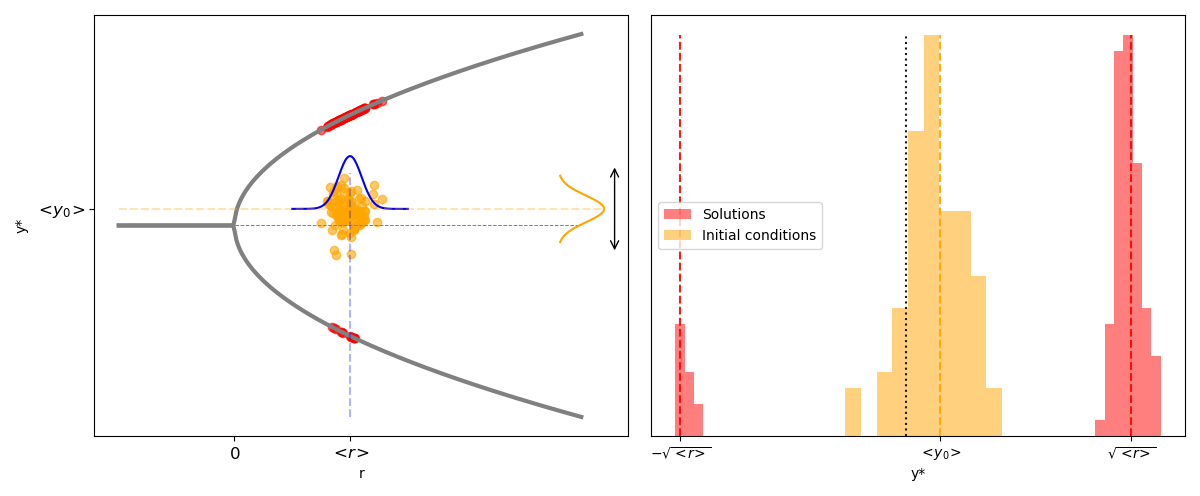
\includegraphics[width=\linewidth]{Images/Metrics/pitchfork_explanation.png}
	\caption{Scheme of the pitchfork transition. The stable branches of the bifurcation diagram are shown in gray solid line. A set of initial conditions with Normal distribution with mean value $<y_0>$ is in orange. Each of these initial conditions is then integrated for a given time $t^*$ for a random parameter $r$ obtained from sampling a normal distribution of mean $<\!r\!>$ and variance $\Delta r$. 
		The results of this integration gives the set of final solutions shown in red. 
		By moving $<\!y_0\!>$ between the stable branches, we obtain transition statistics of the set of solutions for each $<\!y_0\!>$.}
	\label{fig:pitch-explanation}
\end{figure}

At each realization, the parameter $r$ and the initial condition $y_0$ are chosen randomly as stated before, and after some integration time $t^*$ (the same for all realizations) the value $y^*$ is saved. 

In this case, the tails of the distributions when approaching the transition are controlled by the integration time $t^*$ due to critical slowing down. 

\begin{figure}[H]
	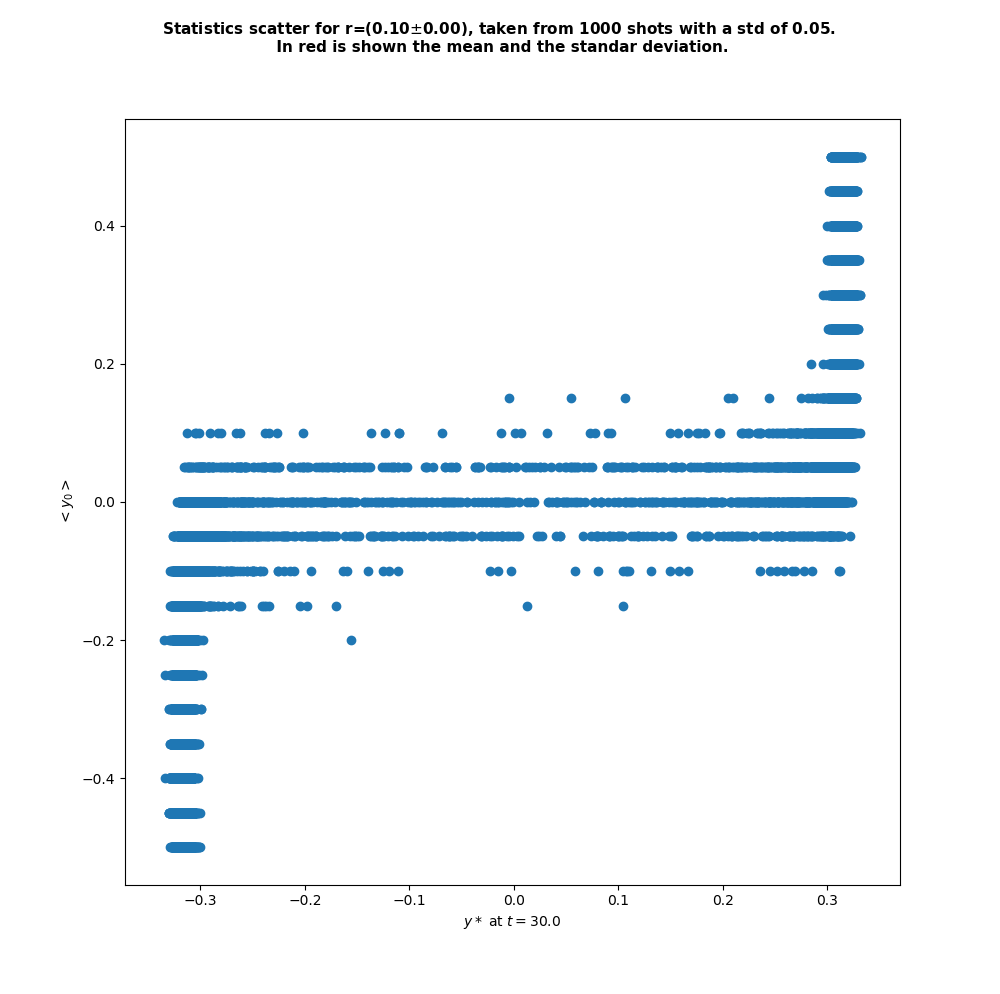
\includegraphics[width=0.3\linewidth]{Images/Metrics/t_30.png}
	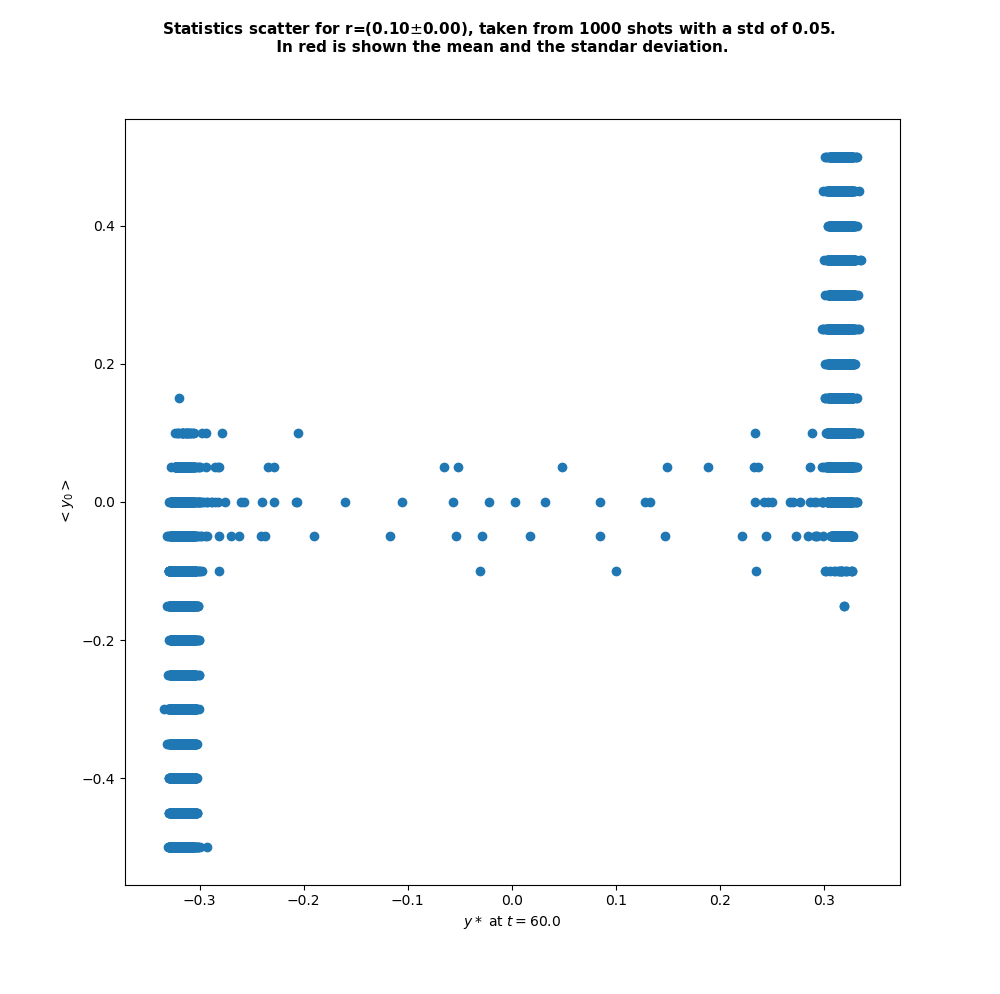
\includegraphics[width=0.3\linewidth]{Images/Metrics/t_60.png}
	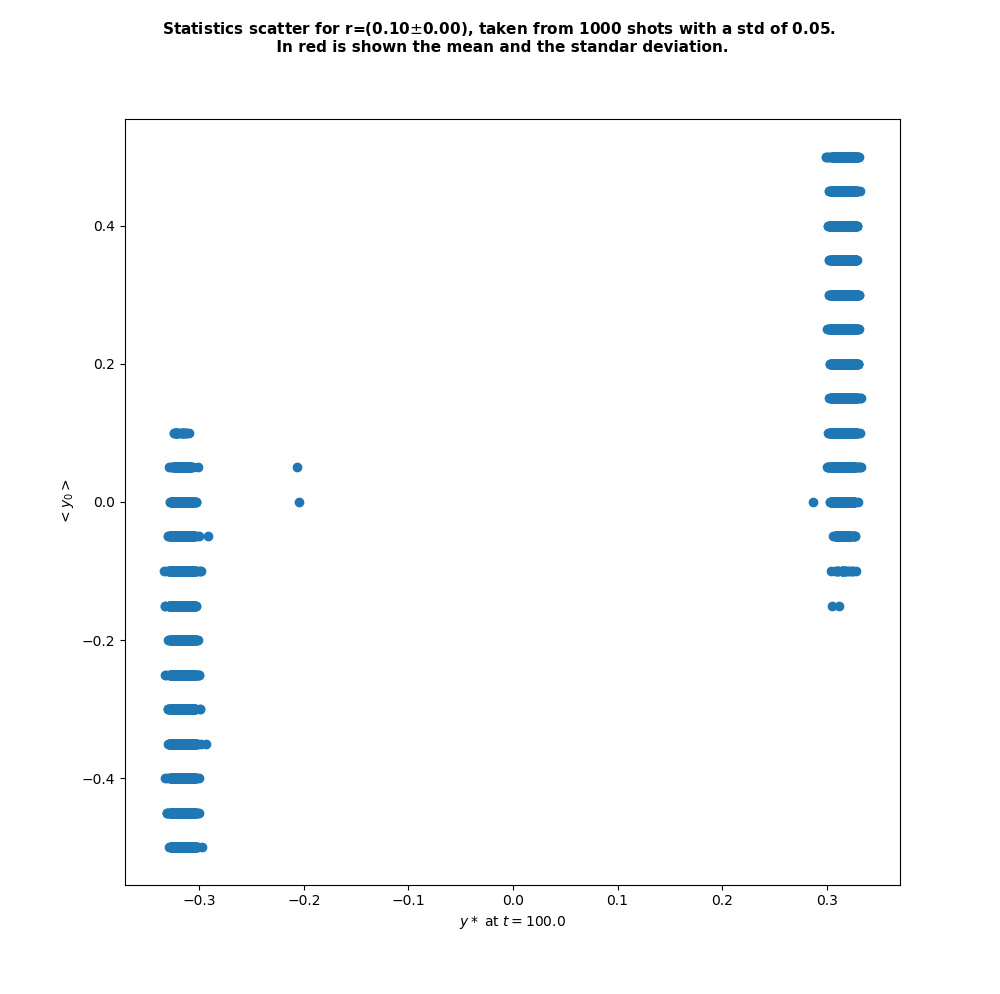
\includegraphics[width=0.3\linewidth]{Images/Metrics/t_100.png}
	\caption{Effect of the integration time on the statistic. The integration times are $t=30, 60, 100$. All other parameters remain constant.}
	\label{fig:critical_slowing}
\end{figure}

This means that the closer the system is to the bifurcation, the more time it takes for a given initial condition to approach the steady state. 
Therefore, for a given integration time $t^*$ the closer the system is to the bifurcation, the more likely it is to 'measure' results far from the stable solutions. 

Figure \ref{fig:critical_slowing} shows the resulting scatter plots for different integration times. In these simulations $<r>=0.1$, $\Delta r=0.003$, and the standard deviation of the initial conditions is $\Delta y_0= 0.05 $ with 1000 points taken for each realization.

\mb{Figure 10: comment on this figure} 

\begin{figure}[H]
	\centering
	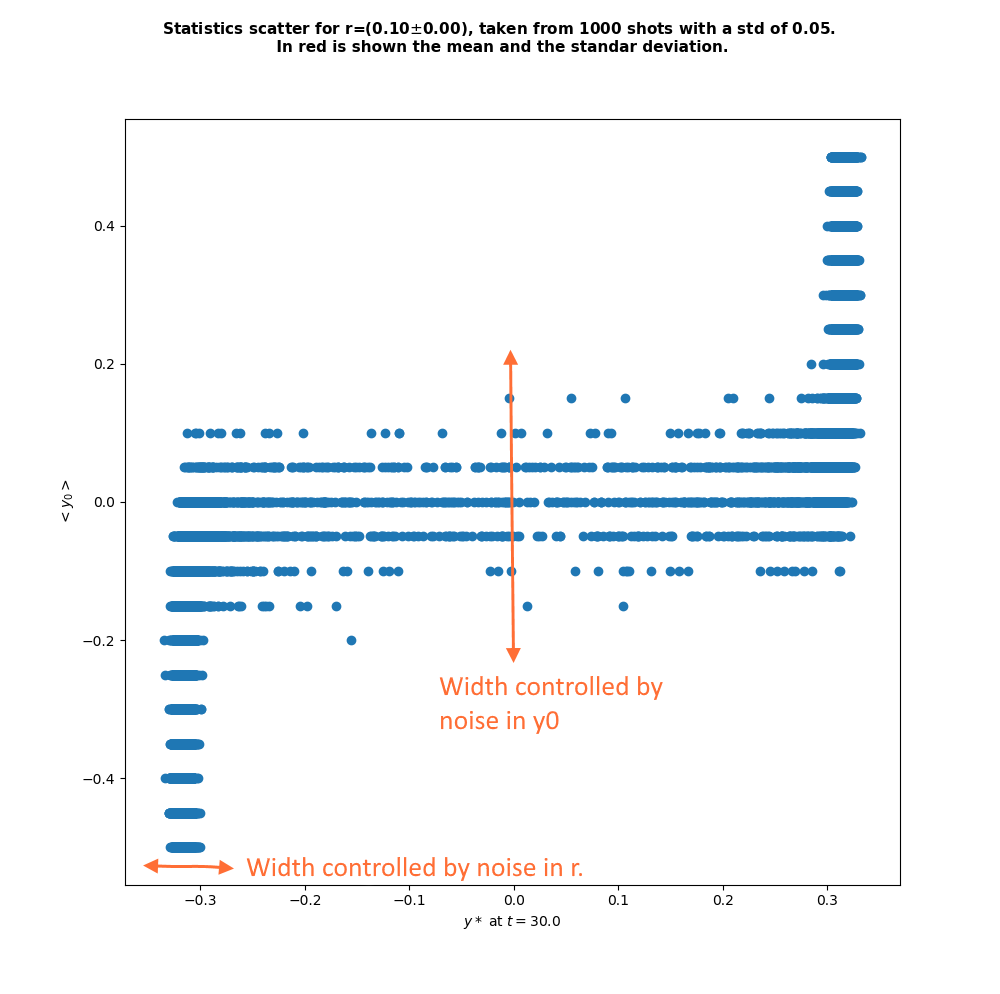
\includegraphics[width=0.4\linewidth]{Images/Metrics/Parameters.png}
	\caption{Effect from critical slowing down.}
	\label{fig:parameters}
\end{figure}
\section{paradox?}



Coming back to the system from eq.~\ref{eq: simplecase}; we can exchange time and control parameter since $\lambda=c_\lambda t+\lambda_0$,and  $\int_{\lambda_0}^{\lambda(t)} \frac{d\lambda}{\dot \lambda}=\frac{\lambda-\la_0}{c_\lambda}$ so 

\begin{equation}
	\lim_{\lambda\to\lambda_c=0} Var[x]=\frac{\sigma^2}{2 |\lambda|}(1-e^{2\frac{\lambda^2}{c_\lambda}})=\frac{\sigma^2}{2 |\lambda|}(2\frac{\lambda^2}{c_\lambda}-\frac{(2\lambda^2/c_\lambda)^2}{2}+\frac{(2\lambda^2/c_\lambda)^3}{6}-\dots)=0
	\label{eq: ST_wellexample}
\end{equation}
\textcolor{red}{correct this.}

\section{Stochastic adiabatic timescale}
\label{apx:sameinit}


\begin{figure}[htb]
	\centering
	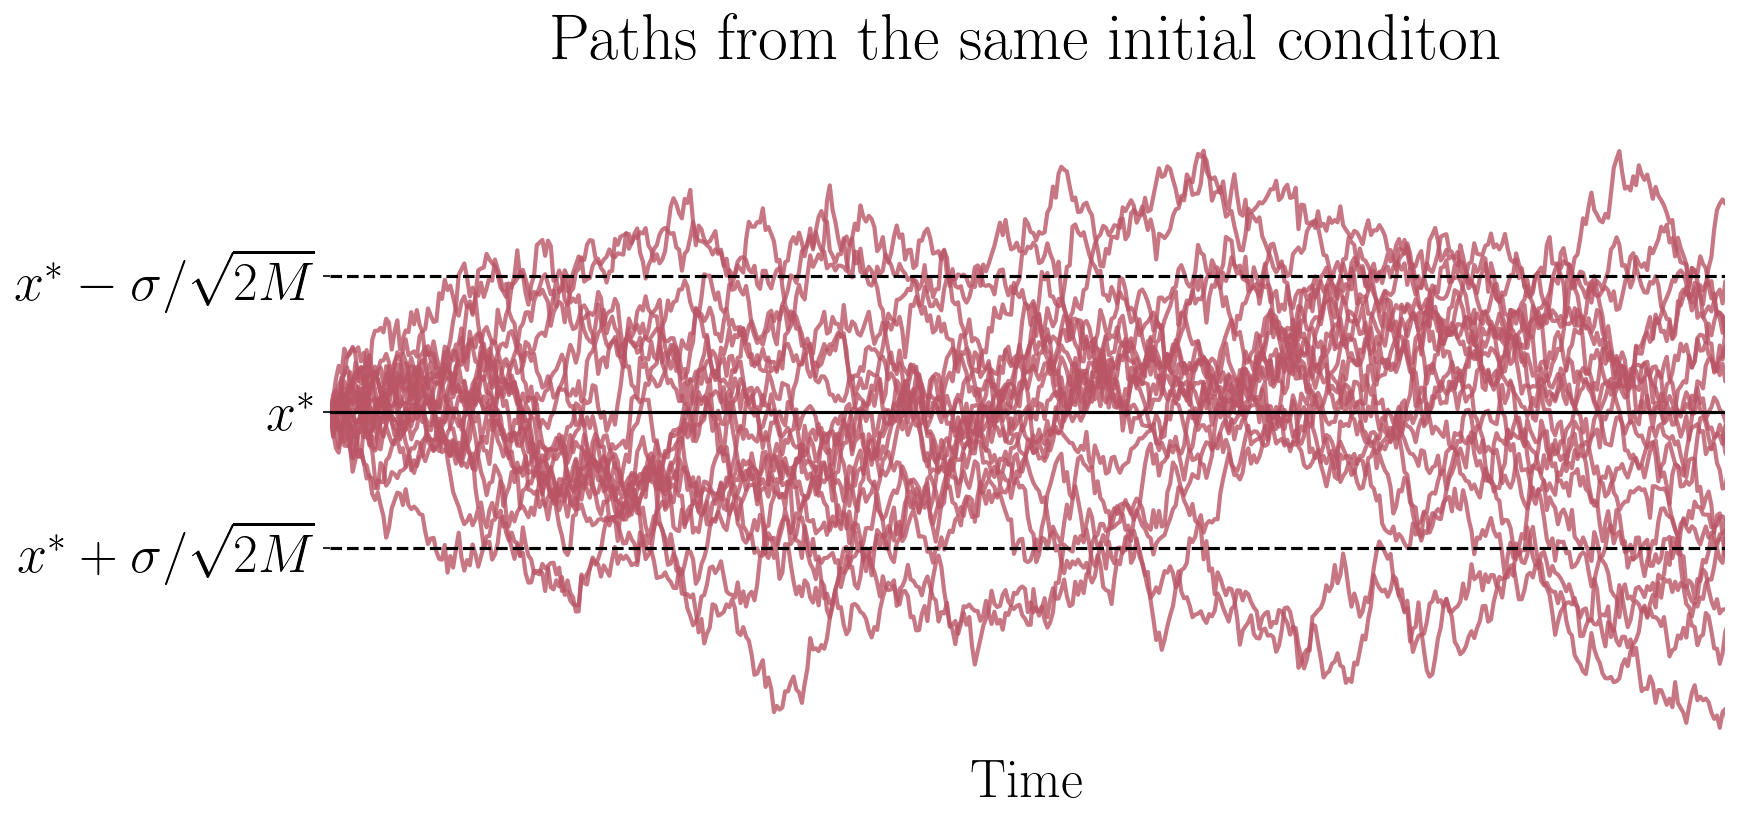
\includegraphics[width=0.9\linewidth]{Images/Metrics/same_init2}
	\caption{20 integrations of}
	\label{fig:sameinit}
\end{figure}



\begin{figure}
	\centering
	\includegraphics[width=0.9\linewidth]{"../Programing Proyects/EE indicators/Simulations with pdfs to test/Stochastic equations/SDE tests jupyter/image_variance_speed/x0_0_tests/toghether/000_variance_test_speed_toghether"}
	\caption{}
	\label{fig:000variancetestspeedtoghether2}
\end{figure}



\begin{figure}
	\centering
	\includegraphics[width=0.9\linewidth]{"../Programing Proyects/EE indicators/Simulations with pdfs to test/Stochastic equations/SDE tests jupyter/image_variance_speed/x0_0_tests/toghether/016_variance_test_speed_toghether"}
	\caption{}
	\label{fig:016variancetestspeedtoghether}
\end{figure}



\section{Extreme events}

Extreme events are unexpected events, both in amplitude and by appearance, compared to the typical dynamics of a system, and might have big consequences. 
By definition,  this events are related to 'heavy tails' on the probability distribution function (PDF) of the systems, that is to say, events that are different to the mean behavior of the system but also rare. 

There are several definitions for extreme events in the literature depending on the subject, but the broad implications and applications they have makes their study interesting. 
This  can range from  extreme events in finance, where they are typically called Black swans or Dragon kings depending on their characteristics \cite{..}, like financial crisis, big fluctuation in the market\cite{bibid}, or bubble bursts\cite{bibid}; to rogue ocean waves that bring down cargo ships \cite{..}, large earthquakes \cite{bibid}, extreme weather\cite{bibid}, population dynamics\cite{bibid}, degree distribution in complex networks\cite{Eom2015}, internet trafic \cite{Hernandez-Campos},  and many more.

Each system can have a different mechanism by which this extreme events are possible, but typically this are due to intrinsic nonlinear responses of the system. 

Some examples of this are self-focusing of ocean waves\cite{..} or laser intensity profiles \cite{..}, large amplitudes due to unlikely explorations of chaotic systems \cite{..}, large fluctuations on systems going through critical transitions \cite{..}.

The study of such events is not only useful for the understanding of their emergence and the feasibility of their forecast. 
But the way a system responds to fluctuations can give us information about some intrinsic properties of a system. 


Given this \textbf{zoo} of behaviors it is clear that a key problem when studying this systems is our capacity to know how they might behave, in particular when they can display big fluctuations or strange or \textbf{freak} behaviors, but also understanding when they can suddenly change their behavior. 

Prediction of freak behaviour, or extreme events, is of particular interest


%add figure of distribution tail. add something on dragon kings and black swans

%\section{Some definitions of extreme events}
%In general, what is defined as an extreme event depends on the field where it happens.
%Some fields have a well defined definition of a extreme events, usually inspired by practicality. 
%
%A common example of this is the definition of Rogue waves from the ocean wave forecast community. 
%In this case a Rogue wave is a wave that is larger than two times the Significant wave height ($H_s$) of the distribution of wave heights in a given \textit{sea state} (a well defined state of sea dynamics). 
%% it would be nice to find a definition of sea state in the bibliography
%Where the significant wave height is defined as the median of the highest $1/3$ \footnote{Defined by taking the median highest 3rd of the data points. for example, for 30000 data, the highest 10000} of the wave height distribution.
%
%A linear theory of wave dynamics with waves following a normal distribution would imply a Rayleigh distribution of wave heights \cite{Onoratoterview}
%
%\begin{equation} 
%	\rho(x,\sigma)=\frac{H}{4\sigma^2}e^{-\frac{H^2}{8\sigma^2}}
%\end{equation}
%
%For a Rayleigh distribution this is aprox $4\sigma$   or  $1.4 \text{RMS(H)}$ \cite{ONORATO201347} \footnote{This is not the same as 4 times the deviation of the Rayleigh distribution $\text{VAR(Rayleigh)}=(8-2\pi)\sigma^2$ . }

%This in turn has inspired similar definitions on other fields, specially in the nonlinear optics community, where it is used due to similarities of both systems \cite{optics nd rogue waves}.

\section{Extreme events from mathematics}
%this is awfully written
From the mathematical side, the field of Extreme event theory(EVT)\cite{some book} has a clear definitions for what it means that a distribution is either fat tailed or heavy tailed.

In this field a a heavy-tailed  (PDF) is a distribution with a “tail” that is \href{http://users.cms.caltech.edu/~adamw/papers/2013-SIGMETRICS-heavytails.pdf}{“heavier” than an Exponential}.

$P(x)$ is a \underline{heavy-tailed} distribution for all $\lambda>0$, 

\[ \lim_{x\to\infty} e^{\lambda x}\bar{F}(x)=\infty\]

with $\bar{F}\sim x^{-1/\xi}$ where $\xi$ is defined as \href{https://math.stackexchange.com/questions/2357673/definition-of-tail-index-of-a-probability-distribution}{the \underline{fat-tail index}}.


discuss 	\href{https://docs.google.com/document/d/18AisjULqnRvs4i_ccdxvNVnvlEr9JIaeGdjIoH_cKEA/edit}{Heavy tailed properties}: Scale invariance, 'catastrophe principle', blow up residual life. 

A distribution is scale invariant if and only if it is Pareto.
%\end{itemize}



Extreme event theory(EVT) has a theorem much like the central limit theorem where it can be shown that under some treatment it is possible to show that the distributions of the tails of any system will converge to a family of Extreme Event distribution functions. 

This fundamental result .... 


Being $s=(x-\mu)/\sigma$ the standardized variable, where $\mu$ is the location parameter, and $\sigma>0$ the scale parameter; EVT shows that the distribution of block maxima of  independent and identically distributed random variables has to converge to 

\begin{equation}
	\begin{aligned}
		f(s,\xi) =  &   e^{-s}e^{-e^{-s}}  \qquad \mathrm{for } \quad \xi =0 \\
		&  (1+\xi s  )^{(-1+1/\xi)} e^{-(1+\xi s)^{-1/\xi}}  \qquad \mathrm{for } \quad \xi \neq0 \quad\mathrm{ and }\quad \xi s >-1 \\
		&  0  \qquad \mathrm{otherwise } \\
	\end{aligned}
\end{equation}

where $\xi$ is the shape parameter.

\section{Bootstraping exponential }
\label{apx:boots}

Same analysis presented in 	\ref{sec:EWS_boots} and \ref{sec:EWS_convergence} for an exponential distribution with scale parameter $1$.

\begin{figure}[htb]
	\centering
	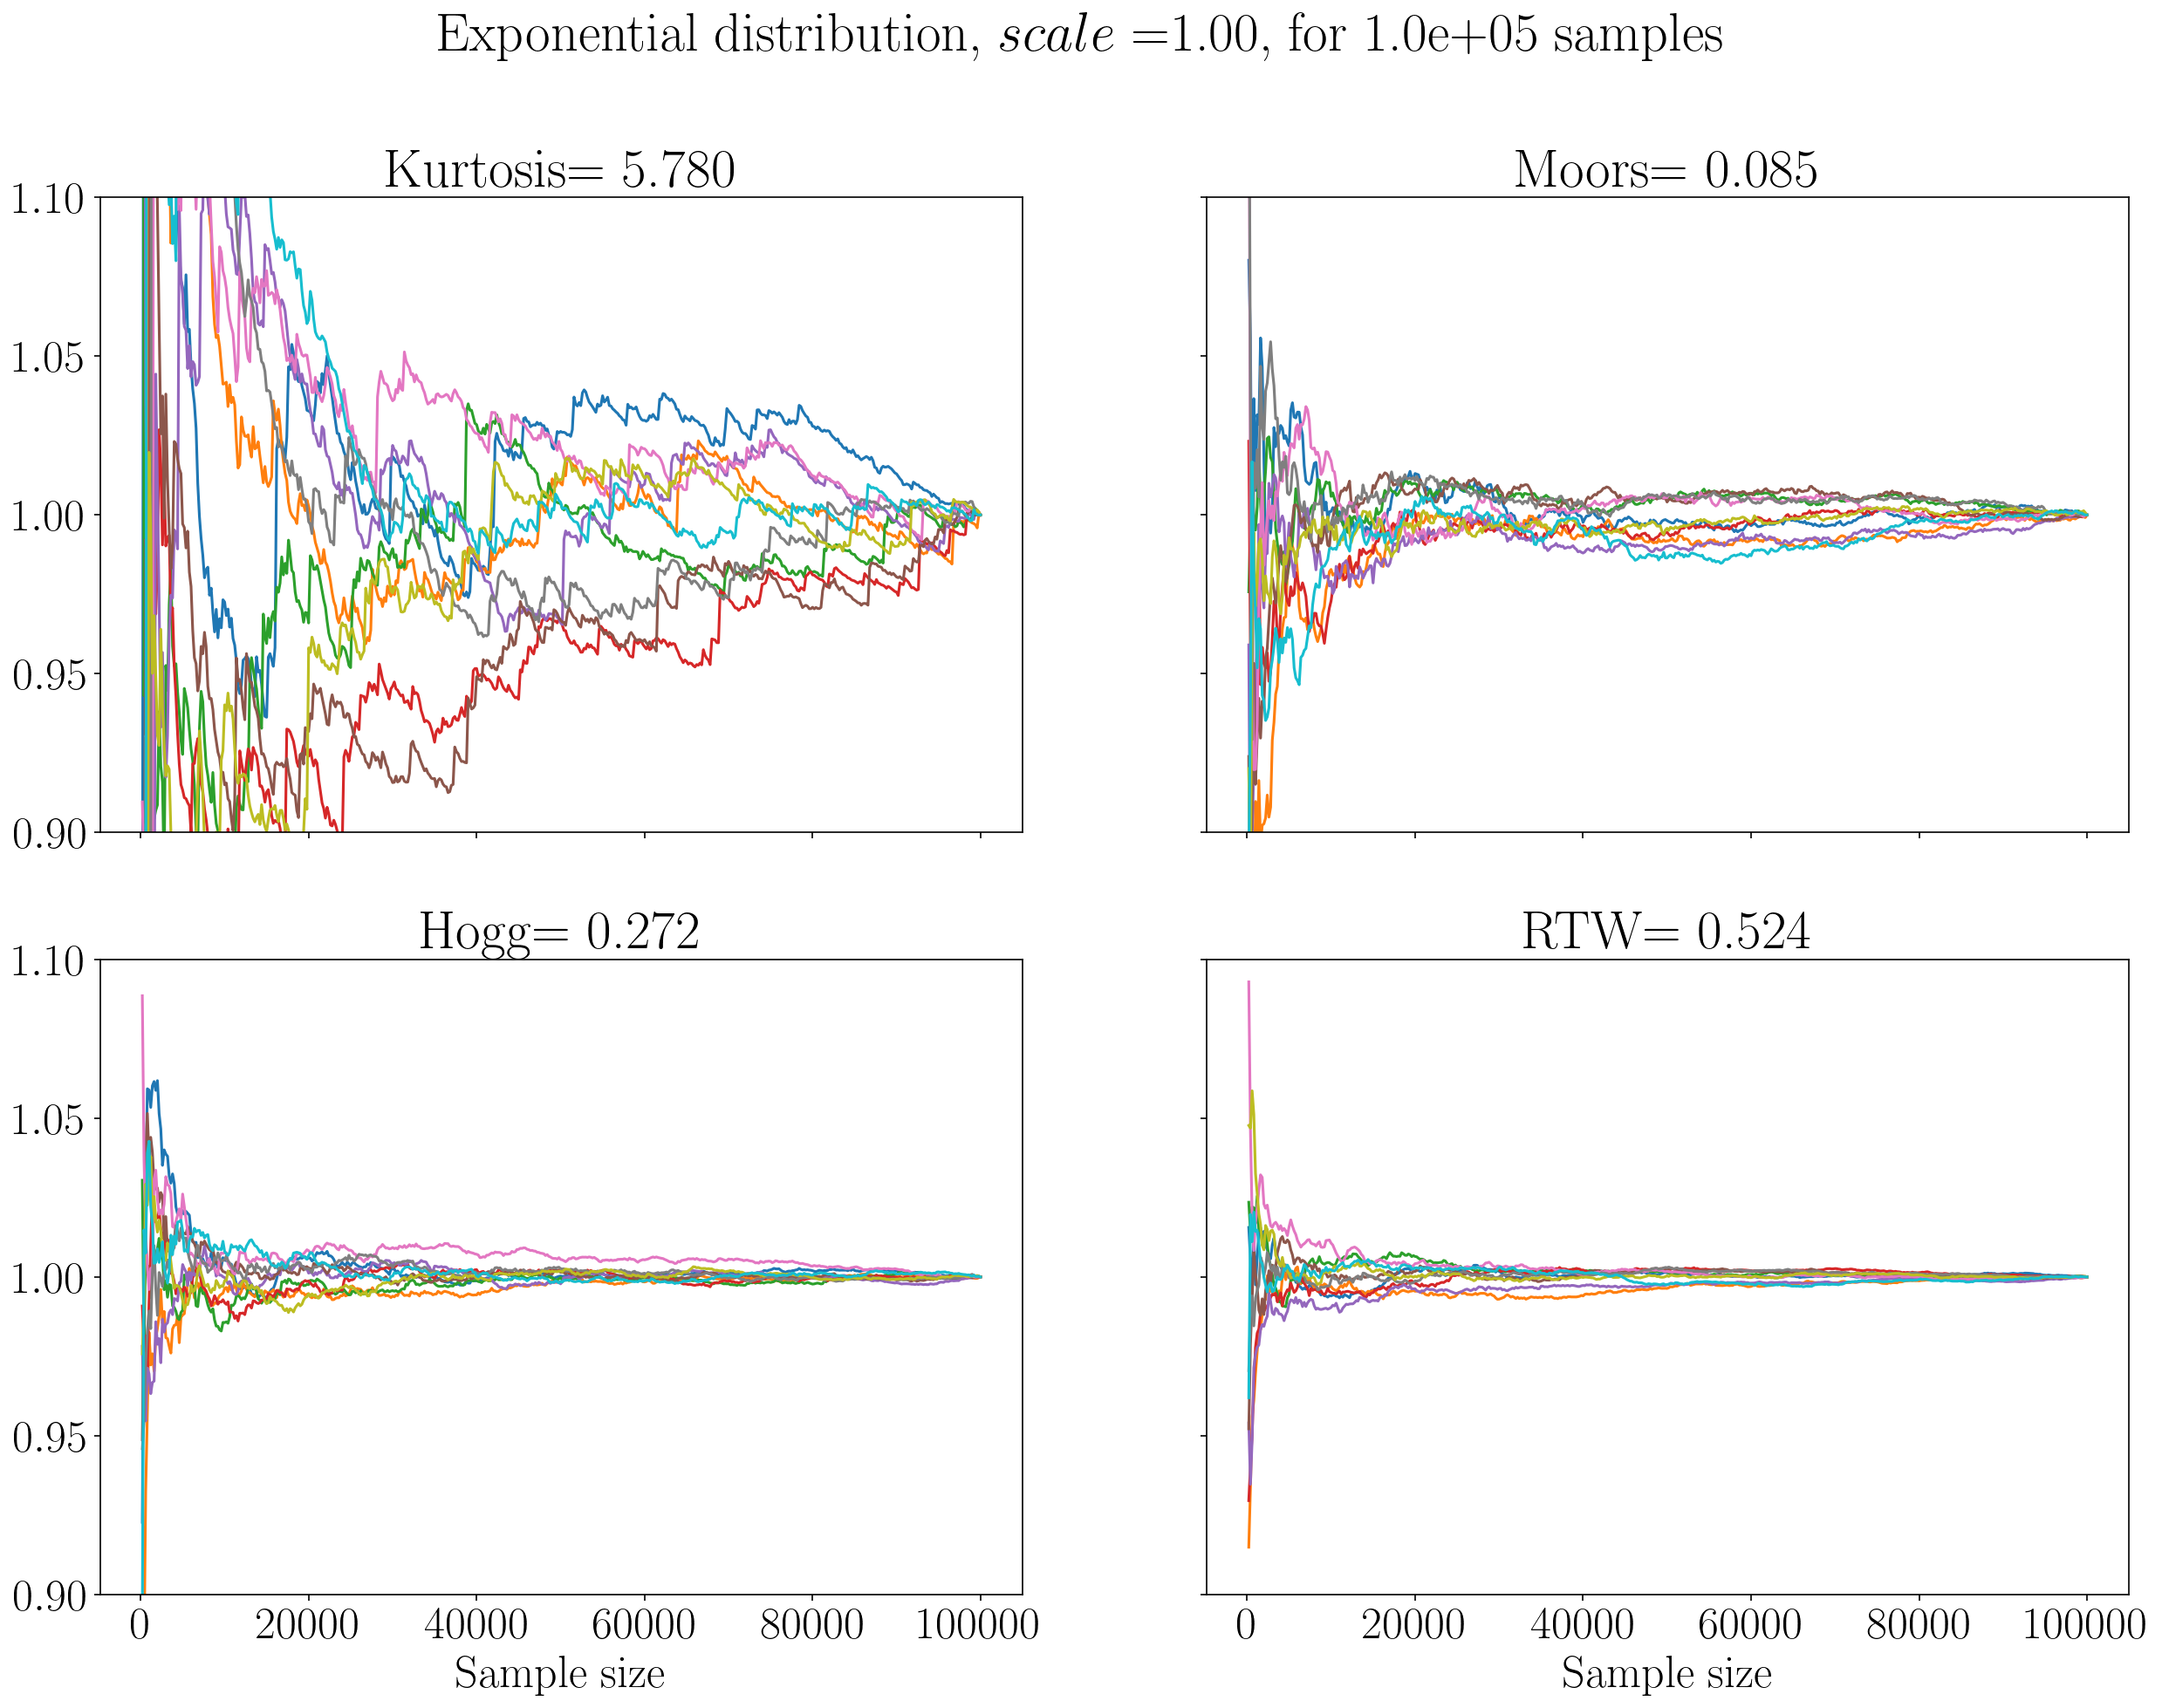
\includegraphics[width=\linewidth]{Images/Metrics/boot_exponential_convergence}
	\caption{ Evolution of the tail statistics: Kurtosis, Moors, Hogg and RTW calculated for an exponential distribution of sample size $10^5$. 
		Each statistic is calculated every $200$ samples. After this is over for all the sample length, the original sample is scrambled and the same procedure is done. This is to show how fast this statistics converge and how much they might fluctuate due to an update of the sample. 
		Each statistic is calculated without correcting for the Gaussian value (ie. is calculated on  the kurtosis, not the excess kurtosis, etc.. ) and normalized to the final value. Only the title values are calculated corrected for the Gaussian values as defined above.}
	\label{fig:bootexponentialconvergence}
\end{figure}

Figure \ref{fig:bootexponentialconvergence} shows the convergence is in statistics doing the same procedure as \cref{fig:convergence_1}, while \cref{fig:boothistogramsexponential} show the same analysis as \cref{fig:Boots_example}.

\begin{figure}[htb]
	\centering
	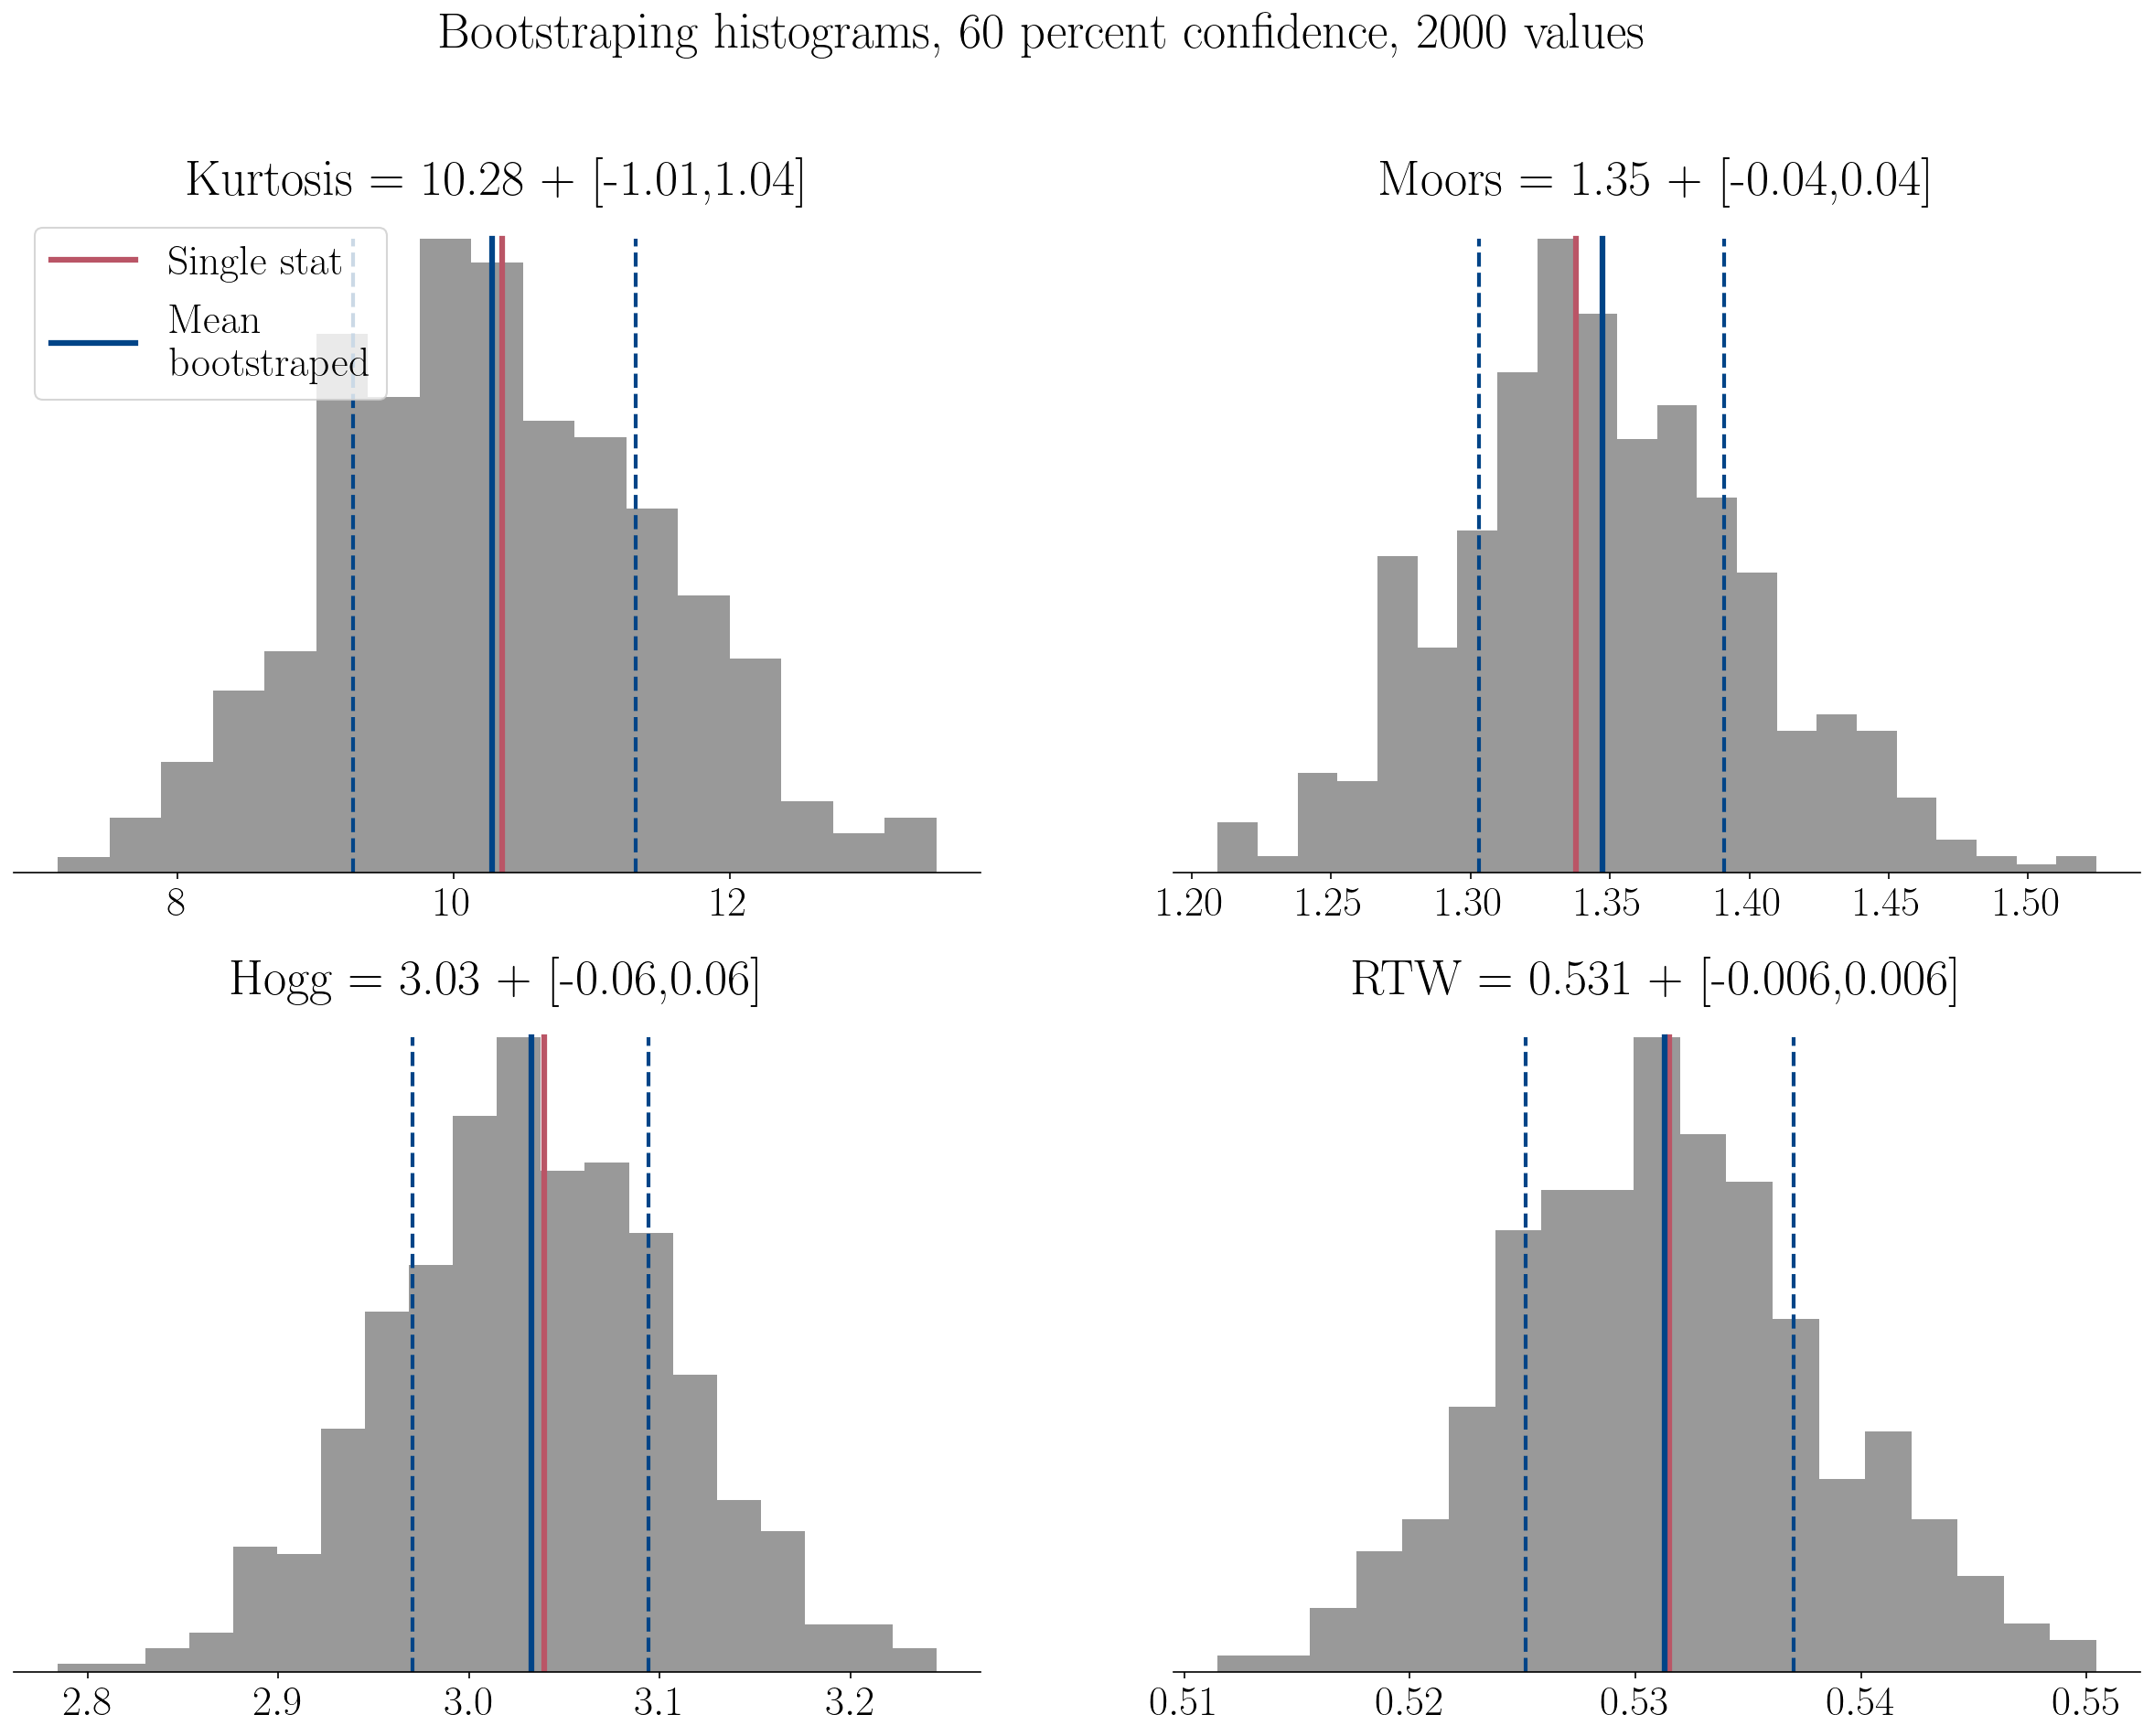
\includegraphics[width=\linewidth]{Images/Metrics/boot_histograms_exponential}
	\caption{ Bootstrapping examples applied to an exponential distribution with 2000 samples, after 600 resamples. The red line indicates the statistic calculated from bootstraping, while the blue line is calculated from the samples, dashed blue indicates the 0.2 and 0.8 percentiles.}
	\label{fig:boothistogramsexponential}
\end{figure}



\section{leftover}

\textbf{Threshold definitions}:
\begin{itemize}
	\item From Ocean Dynamics: $H_f=2H_s $
	\item From Ocean Dynamics (with the definition given above): $H_{m0}=8\sigma$
	\item From Ocean Dynamics: $H_{rms}=2\times 1.4 \text{RMS(H)}$
	\item From Data Minning and descriptive statistics outliers:
	
	$$adj_l=Q_1-1.5r \qquad \qquad adj_H=Q_3+1.5r$$
	
	\item From a talk with Jerome: Another way to define the thresholds could be to make two symmetric distributions based on the original, for each side of the mean. And the take as a threshold some multiple of the standard deviation of this distributions. 
	
	For example, if we want to recover the same value as using $2H_s$ for a Rayleigh distribution, then the new threshold would be the mean of the distribution plus \textbf{$3.69$} times the standard deviation of a symmetrical distribution taken from the right side. 
	
	This way the low intensity threshold can be defined as  the mean od the distribution minus \textbf{$3.69$} times the standard deviation of a symmetrical distribution taken from the lef side, as shown in fig \ref{fig:symthreshrayl} . 
	
	\begin{figure}
		\centering
		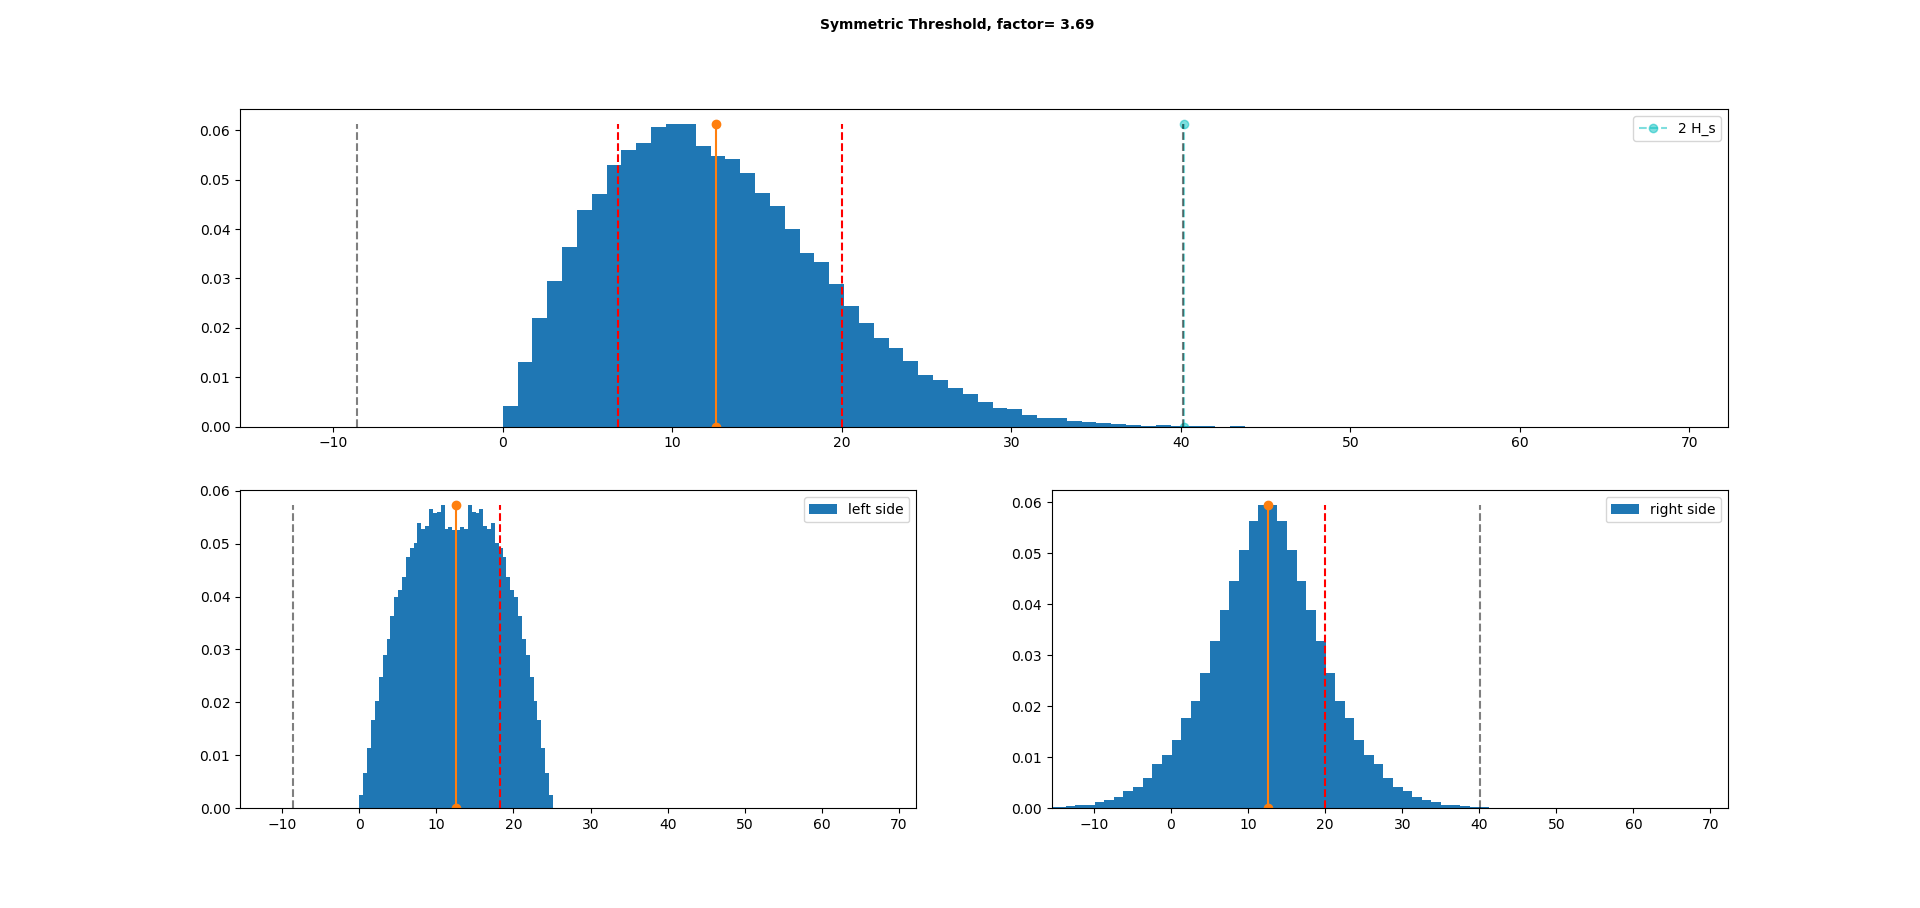
\includegraphics[width=0.8\linewidth]{Images/Metrics/sym_thresh_rayl}
		\caption{Example of the symmetric thresholds for a Rayleigh distribution.}
		\label{fig:symthreshrayl}
	\end{figure}
	
\end{itemize}	

\section{Non equilibrium variance}
\label{apx:variance_contradiction}

At the bifurcation, if the eigenvalues of the Jacobian matrix are real, them $M(x^*,\lambda_c)=0$, this bring forward a possible paradox: \textbf{the equilibrium variance \eqref{eq: ST_variancelim} diverges at $\lambda_c$, but looking at the out of equilibrium factor, it goes to $0$, so the variance might not only not diverge but even vanish at the bifurcation.  }


\begin{equation}
	\lim_{\lambda\to\lambda_c} Var[x]=\frac{\sigma^2}{2 ||M(x^*,\lambda)||}(1-e^{-2M(x^*,\lambda)	\int_{\lambda_0}^{\lambda(t)} \frac{d\lambda}{\dot \lambda}})=\frac{"0"}{"0"}
	\label{eq: ST_lamblim}
\end{equation}

We will see with a simple example that what happens here is that, since we arrive at the bifurcation at a finite time due to the sweeping parameter, the variance of the ensemble is actually finite. 


	\section{Upper constraint of the integration scheme.}
	\label{apx:param_speed_integration}
	
	In the integration scheme there is a limit to how big the time step can be, given a relaxation time $t^*=||M||^{-1}$.
	
	If the time step ($\Delta t$) is larger than the relaxation time ($t^*$) then the system cannot relax to the equilibrium stable ($x^*$) and it becomes unstable.
	
	\begin{figure}
		\centering
		\begin{tikzpicture}
			\node (time) at (11,0)  [right]{$t$};
			\draw [->,very thick,black](0,0) -- (11,0);
			\node[above,left] at (0,3) {a)};
			\foreach \i in {0,...,4}
			{ \draw (2*\i,0) node[rectangle, thin,left color=col2, right color=white!,shading angle=180,anchor=south west, minimum height=3cm,minimum width=2cm,opacity=0.2+\i*(1-0.2)/9] () {}; }
			\foreach \i in {0,...,5}
			{ \filldraw (2*\i,0) circle [circle,black,fill=black,align=center,radius=0.05cm] ; }
			\node[below] (a) at (0,0) [center,below]{$t_i$};
			\node[below] (b) at (2,0) [center,below]{$t_{i+1}$};
			\node[below] (b) at (4,0) [center,below]{$t_{i+2}$};
			\draw [dotted , thick , black,right](6,-0.3) -- (8,-0.3);
			\node[below] (b) at (10,0) [center,below]{$t_{n}$};
			\tzfn[->,col1,ultra thick]{3.5*exp(-1.3*\x)}[0.1:1.5]{}[al]		
		\end{tikzpicture}
		
		\begin{tikzpicture}
			\node (time) at (11,0)  [right]{$t$};
			\draw [->,very thick,black](0,0) -- (11,0);
			\foreach \i in {0,...,9}
			{ \draw (1*\i,0) node[rectangle,  thin,left color=col2, right color=white!,shading angle=180,anchor=south west ,anchor=south west, minimum height=3cm,minimum width=1cm,opacity=0.2+\i*(1-0.2)/9] () {}; }
			\foreach \i in {0,...,10}
			{ \filldraw (1*\i,0) circle [circle,black,fill=black,align=center,radius=0.05cm] ; }
			\node[below] (a) at (0,0) [center,below]{$t_i$};
			\node[below] (b) at (1,0) [center,below]{$t_{i+1}$};
			\node[below] (b) at (2,0) [center,below]{$t_{i+2}$};
			\draw [dotted , thick , black,right](6,-0.3) -- (8,-0.3);
			\node[below] (b) at (10,0) [center,below]{$t_{n}$};		
			\tzfn[->,col1,ultra thick]{3.5*exp(-1.3*\x)}[0.1:1.5]{}[ar]
			\node[above,left] at (0,3) {b)};	
		\end{tikzpicture}
		\caption{a) Small $\Delta t$. b) Big $\Delta t$. For a given value of $t^*=||M(\lambda)||^{-1}$ the system has a well defined relaxation timescale. Ideally the times array should change slow enough for the system to be able to 'relax'.}
		\label{fig: velocity_param2}
	\end{figure}
	
	
	Therefore we choose $ \Delta t < min(t^*)/2 $ where $min(t^*)$ is the smallest relaxation time over the evolution of the parameter $\lambda$.
	Thus the $\Delta t$ is determined by the region with highest \textit{resilience}, far from the b-tipping bifurcation. 
	
	$t_{var}=\frac{1}{2M}=min(t^*)/2$
	
	
	$ \Delta t < min(t^*)/4 $
	


Warning of a forthcoming collapse of the Atlantic
meridional overturning circulation

On Conditions for Rate-induced Tipping in Multi-dimensionalDynamical Systems


\subsection{Sharp transition mockup}	
\label{ewsapx: transition}
%\ag{Describe the data: simulated data for each numerical experiment; Goery's data, filament data [with Experimental setup if we want to include them.]}

Since we want to have a data set where we can control the 'tailedness' of the distribution, we will use a couple toy models thought specifically to have a smooth transition between random data with a normal distribution, to a distribution with an arbitrary large tail. 

We also show the same method applied to a real data set with a phase transition.

\subsubsection{Simulation of an experimental transition.}
The goal of this test is to understand how a signal for a quick transition might look on the tail related statistics. To do this we test adding noise to an Error function.

%simulate what one might see if acquiring data while going through a sharp or smooth transition between two given values.
The noise is added by a background Gaussian noise in the data, and a Gaussian indetermination of the experimental parameter (sampling Gaussian) at which the measurement takes place \footnote{For example: Measuring a transition in conductivity for different temperatures. 
	In this case we suppose there would be a Gaussian fluctuation for the temperature at which we set the experiment, and there is some background noise in the instrument we use to measure the conductivity. }. 
In this case the 'sharpness' transition is controlled by the transition window (the slope of the Erf function) compared to the noise from the sampling Gaussian $\sigma$.

Each data point is generated by 
\begin{equation}
	\mathrm{Erf}(z)=\frac{2}{\sqrt{\pi}}\int_0^z e^{-t^2}
\end{equation}

\begin{equation}
	y_j=A_0\left(\mathrm{ Erf} \left( \frac{(x_j)}{\sqrt{2}s_2}\right)+1\right)+y_0+n_0
\end{equation}

Where $n_0$ is a random value taken from a normal distribution N(0,$\sigma_{n_0}$), $y_0$ is an offset for the lower value of the Erf function. 
$x_j$ is a random number generated by a normal distribution $N(\mu,\sigma)$, and $S_2$ is  a parameter that controls the slope (and the width of the transition) as shown in figure \ref{fig:transition_example}. 

\begin{figure}[htb]
	\centering
	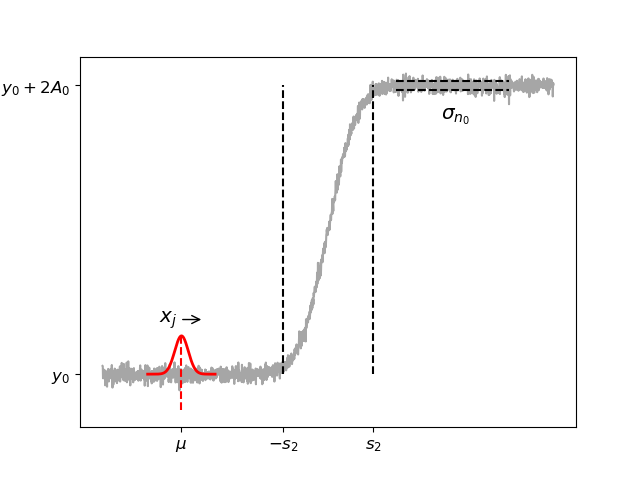
\includegraphics[width=0.7\linewidth]{Images/Metrics/erf_example.png}
	\caption{ Sketch for smooth transition between the mean values $y_0$ and $y_0+2A_0$ using an $\mathrm{Erf}$ function. The dispersion around such values is given by $\sigma_{n_0}$, and the transition occurs between $-s_2$ and $s_2$.
		In red it is shown the sampling Gaussian that simulates an imperfect measurement device or indetermination of an experimental parameter. 
		This example has $\sigma_{n_0}=0.06$, $\sigma=0.6$, $A0=2$ and  $S_2=1$.}
	\label{fig:transition_example}
\end{figure}
Changing the value of $\mu$ is equivalent to acquiring data from a given point in the Erf function, where there is inherent  noise both in the data acquired and the value of $\mu$ for which one acquires the data. 

Therefore acquiring data far from the transition gives a Gaussian result with a variance of $\sigma_{n_0}$, and changes as $\mu$ approaches the transition. 

This gives two parameters to characterize a transition between two values.
$\frac{\sigma_{n_0}}{A_0}$ reflects the relation between the noise and the distance between the steady values $y_0$ and $y_0+A_0$. 
$\frac{\sigma_{n_0}}{A_0}<1$ gives a big transition, while $\frac{\sigma_{n_0}}{A_0}>1$ gives a small transition. $\frac{\sigma}{s_2}$ reflects the relation between the noise of the sampling Gaussian transition length; $\frac{\sigma}{s_2}<1$ gives a smooth transition, while $\frac{\sigma}{s_2}>1$ gives a sharp transition. Such different possible dynamics can be seen in figure \ref{fig:transition_configurations}.
\footnote{\ag{i'm not sure it should be $s_2$ or $2s_2$; and $A0$ or $2A0$.Rta: I think it should be $\sigma/s_2$ and $2\sigma_{n_0}/A_0$ since this gives overlap in the highest $10 \%$  of the gaussians, I need to change the text and simulations at some point to show this. }}.


%\begin{figure}[h]
%\centering
%    	\includegraphics[width=0.45\linewidth]{images/metric/simulation-transition/erf_example_transition_stats.png}
%   	\includegraphics[width=0.45\linewidth]{images/metric/simulation-transition/erf_example_transition_stats2.png}\\
%  	\includegraphics[width=0.45\linewidth]{images/metric/simulation-transition/erf_example_transition_stats3.png}
% 	\includegraphics[width=0.45\linewidth]{images/metric/simulation-transition/erf_example_transition_stats4.png}
%\caption{ Two possible behaviours for the transition statistics, depending on the relation between $s_2$ and $\sigma$. a)$\frac{\sigma_{n_0}}{A_0}$= 0.03 $\frac{\sigma}{s_2}$=2, b)$\frac{\sigma_{n_0}}{A_0}$= 0.03 $\frac{\sigma}{s_2}$=0.6 , c)$\frac{\sigma_{n_0}}{A_0}$= 1.25 $\frac{\sigma}{s_2}$=2,
	%   	d)$\frac{\sigma_{n_0}}{A_0}$= 1.25 $\frac{\sigma}{s_2}$=0.6 . Each histogram is plotted in log scale using a the 'blocks' method from the  %\texttt{astropy.stats.histogram} dependency to be able to better show the long tales. \ag{change the fraction display}}
%\label{fig:transition_configurations}
%first case:  \sigma_n0=0.06, sigma=2, A0=2, S2=1
%second case: \sigma_n0=0.06, sigma=0.6, A0=2, S2=1
%third case:\sigma_n0=2.5, sigma=2, A0=2, S2=1
%forth case:\sigma_n0=2.5, sigma=0.6, A0=2, S2=1
%\end{figure}

\begin{figure}[H]
	\centering
	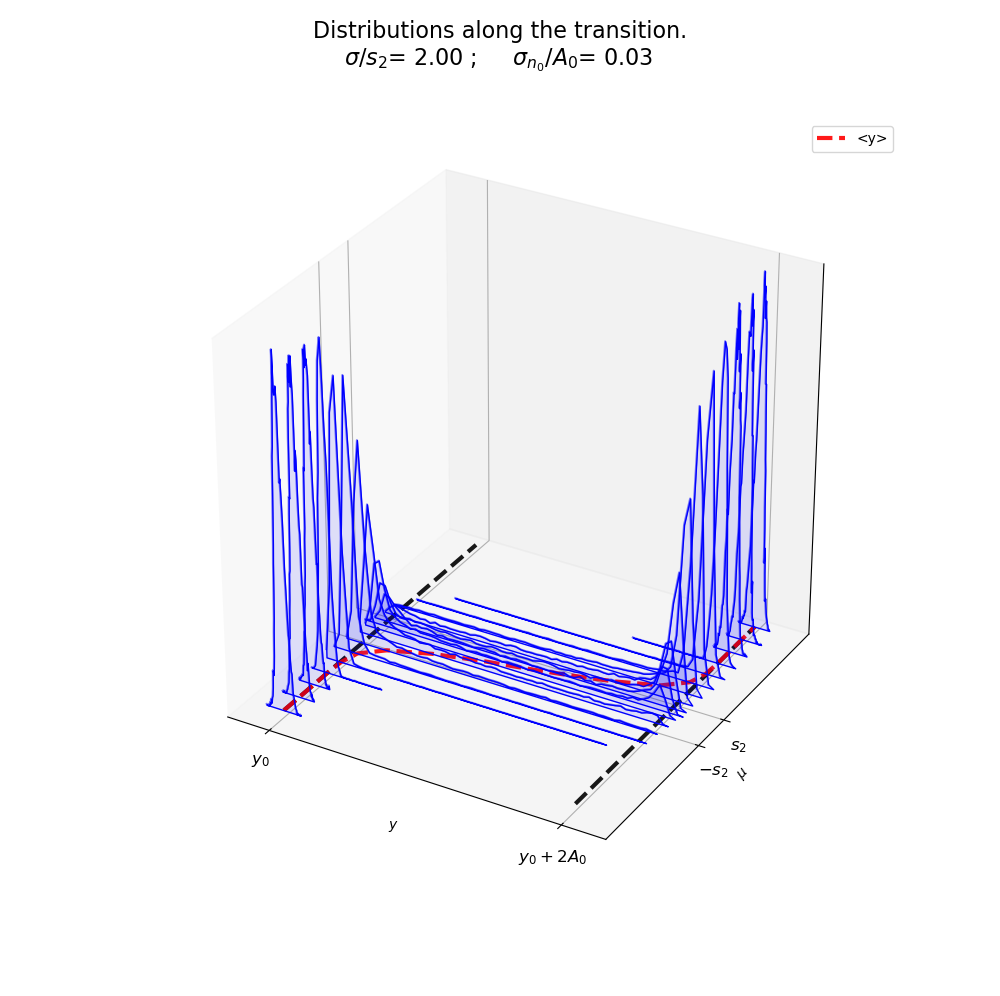
\includegraphics[width=0.45\linewidth]{Images/Metrics/erf_example_transition_stats_3da.png}
	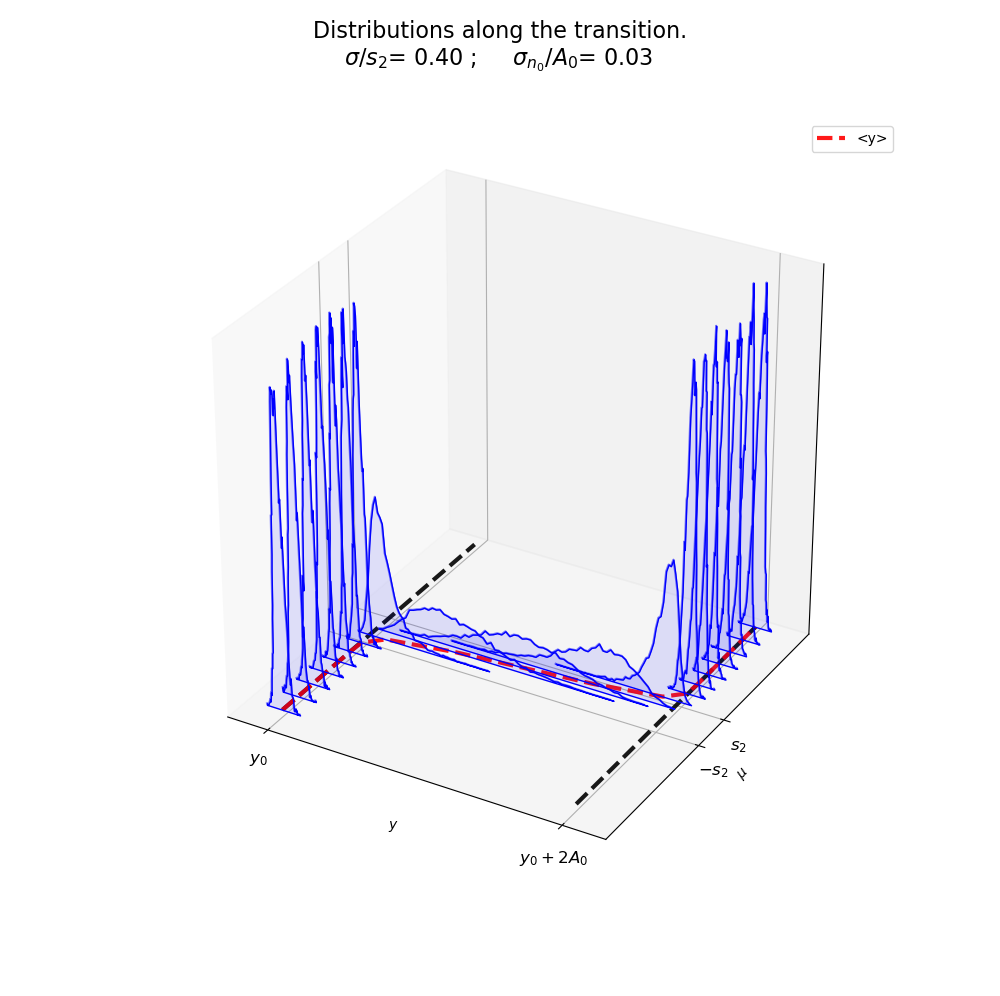
\includegraphics[width=0.45\linewidth]{Images/Metrics/erf_example_transition_stats_3db.png}\\
	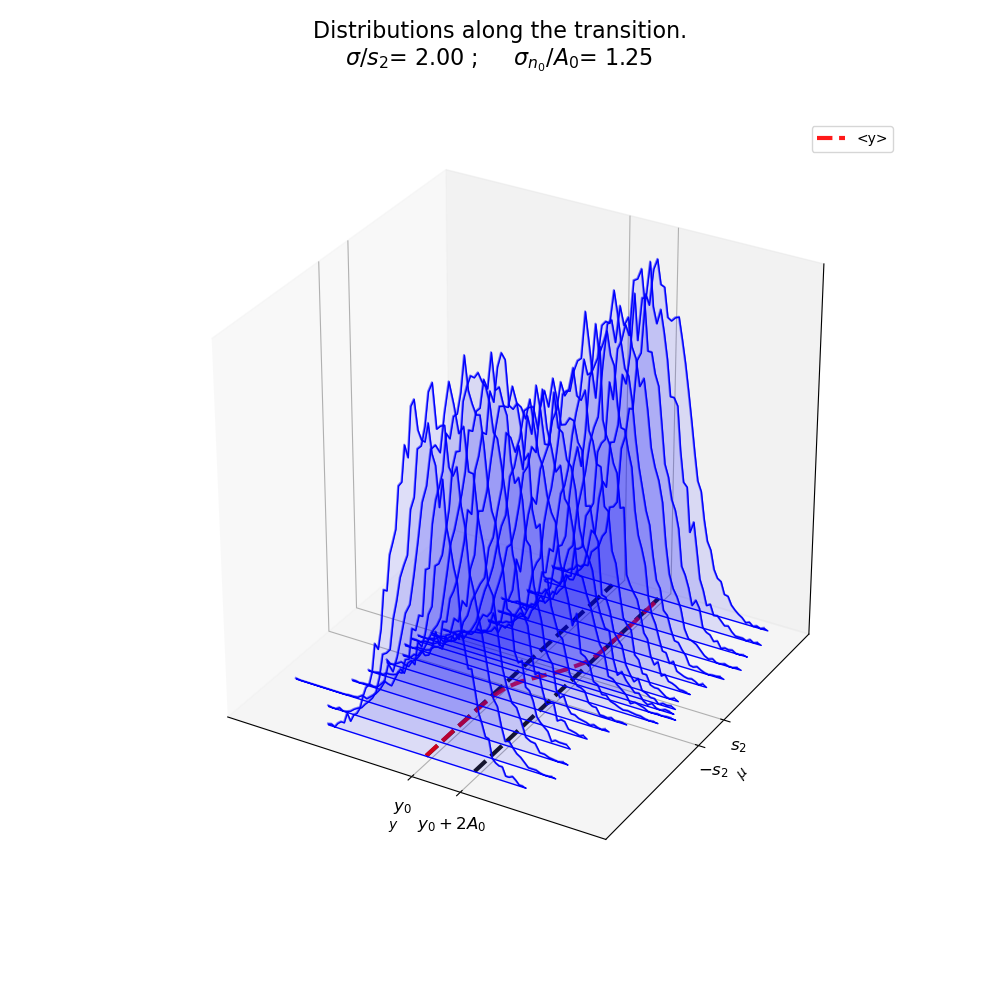
\includegraphics[width=0.45\linewidth]{Images/Metrics/erf_example_transition_stats_3dc.png}
	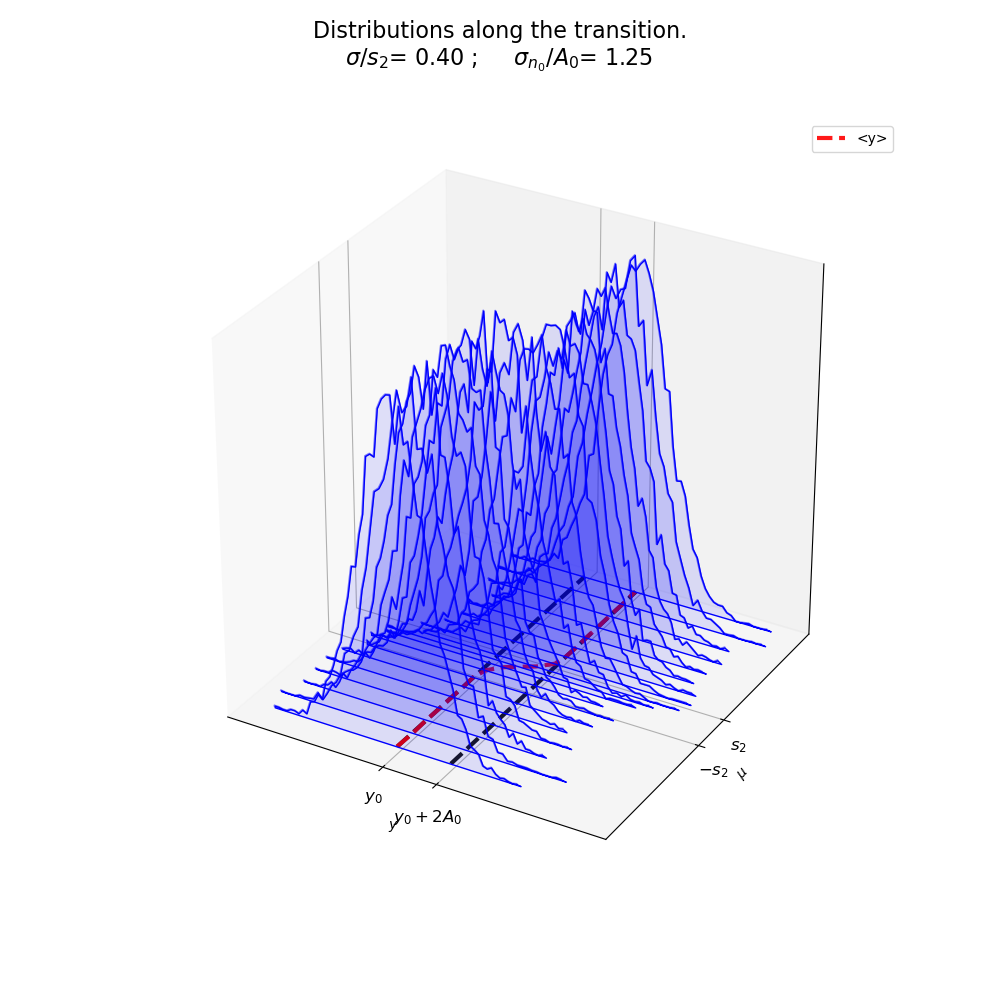
\includegraphics[width=0.45\linewidth]{Images/Metrics/erf_example_transition_stats_3dd.png}
	\caption{ \sout{Two} possible behaviours for the transition statistics, depending on the relation between $s_2$ and $\sigma$. a)$\frac{\sigma_{n_0}}{A_0}$= 0.03 $\frac{\sigma}{s_2}$=2, b)$\frac{\sigma_{n_0}}{A_0}$= 0.03 $\frac{\sigma}{s_2}$=0.4 , c)$\frac{\sigma_{n_0}}{A_0}$= 1.25 $\frac{\sigma}{s_2}$=2,
		d)$\frac{\sigma_{n_0}}{A_0}$= 1.25 $\frac{\sigma}{s_2}$=0.4 . Each histogram is plotted in log scale using the 'blocks' method from the  \texttt{astropy.stats.histogram} dependency to be able to better show the long tales. \ag{change the fraction display} \mb{Use larger font in labels!}}
	\label{fig:transition_configurations}
	%first case:  \sigma_n0=0.06, sigma=2, A0=2, S2=1
	%second case: \sigma_n0=0.06, sigma=0.5, A0=2, S2=1
	%third case:\sigma_n0=2.5, sigma=2, A0=2, S2=1
	%forth case:\sigma_n0=2.5, sigma=0.4, A0=2, S2=1
\end{figure}
For $\mu=0$ (the symmetric case), when  $\frac{\sigma}{s_2}=1$ the resulting distribution is close to a uniform distribution when $\frac{\sigma_{n_0}}{A_0}<1$. This means that the transition between low and high values of $\frac{\sigma}{s_2}$, for $\mu=0$  and low $\frac{\sigma_{n_0}}{A_0}$ is a continuous transition between a Gaussian to a bi-modal distribution, going though a normal distribution.  

Other possibilities to explore for transitions is the extreme case of a heavyside function, or the case where the transition happens in the slope of a linear signal. 


\section{Overshoot tipping with high noise}

A particular case that has not been explore sufficiently in the literature is the case of a moving parameter that returns to it's initial value, goes though a bifurcation of the autonomous system along it's evolution, but also presents some 'high' stochastic noise. 



Here we consider the system 

\begin{equation}
	\begin{cases}
		dx&=(-x^3+0.9x+\lambda)dt+\sigma dW\\
		d\lambda&=2(-(\la_0+\la_{max})/(t_f/2)^2)(t-t_f/2)\\
		\lambda(t_0=0)&=\lambda(t=t_f)=\lambda_0
	\end{cases}
\end{equation} 

Here the speed of the parameter is defined by the final time $t_f$.

With very low noise, the system behaves as in \cref{fig:overshoot2}, however, if we set $\sigma=0.1$ we can see different behaviours due to the stochasticity of the system. 

Figures \ref{fig:overshootnoise4,fig:overshootnoise2,fig:overshootnoise3} show three independent realizations of this system, with the same parameters, where in \textcolor{col1}{yellow} we show a slow sweeping, in \textcolor{col2}{red} an intermediate sweeping and in \textcolor{col3}{blue} a fast sweeping (just like in \cref{fig:overshoot2}). 
However in this case, the intermediate and fast sweeped integration might or might not tip to the lower stable branch depending on the stochastic path the system might take.

\begin{figure}
	\centering
	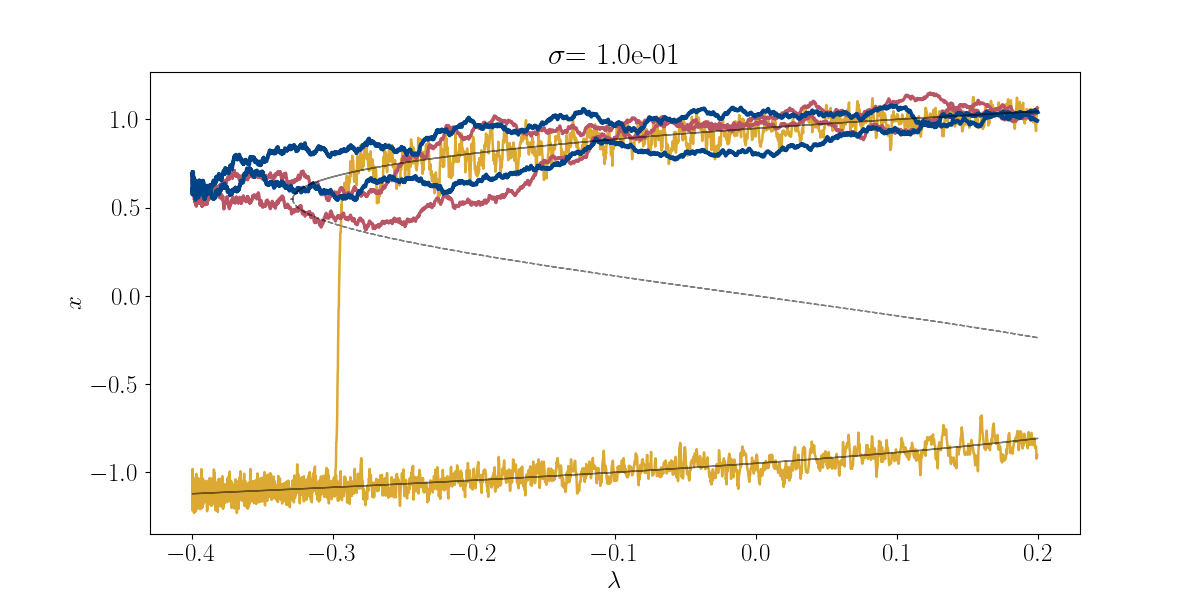
\includegraphics[width=0.9\linewidth]{Images/Metrics/overshoot_noise4}
	\caption{}
	\label{fig:overshootnoise4}
\end{figure}

\begin{figure}
	\centering
	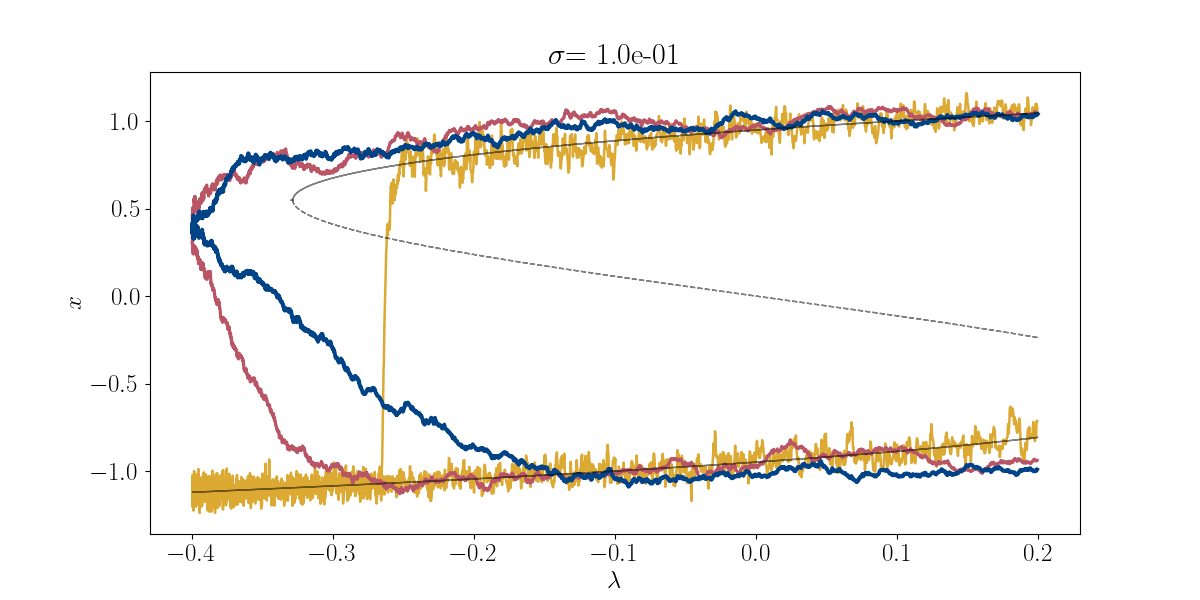
\includegraphics[width=0.9\linewidth]{Images/Metrics/overshoot_noise2}
	\caption{}
	\label{fig:overshootnoise2}
\end{figure}

\begin{figure}
	\centering
	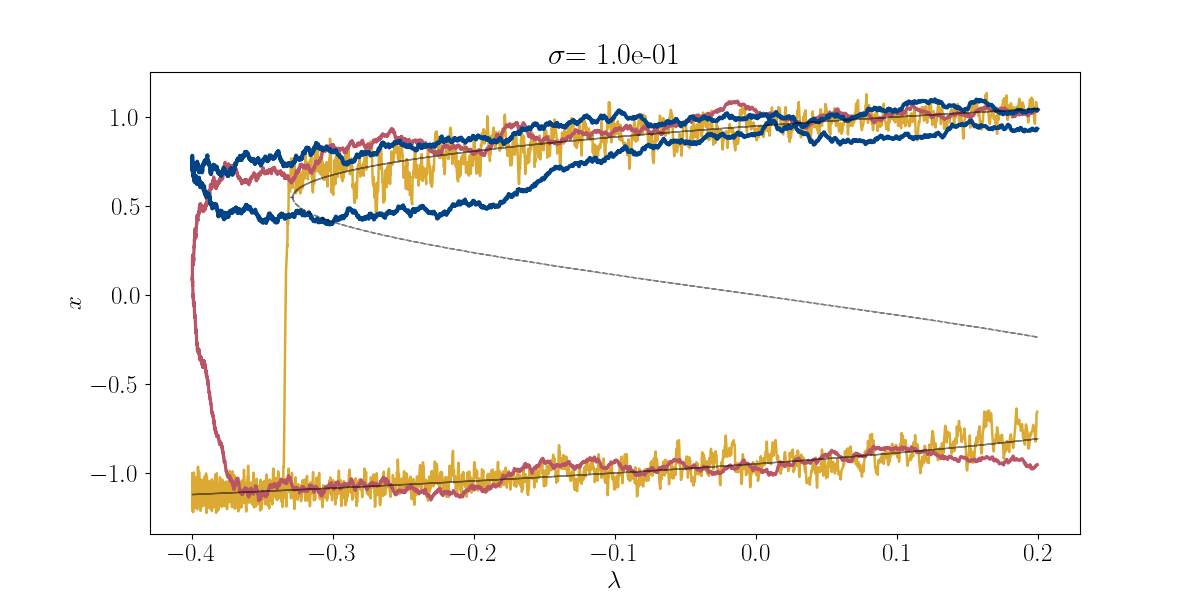
\includegraphics[width=0.9\linewidth]{Images/Metrics/overshoot_noise3}
	\caption{}
	\label{fig:overshootnoise3}
\end{figure}

\Cref{fig:overshootnoise4} shows a case where neither the fast and intermediate sweeped parameters tip, while \cref{fig:overshootnoise2} show both cases tipping, and \ref{fig:overshootnoise3} shows the intermediate sweeped parameter tipping while the fast parameter does not, as in the deterministic systems.  

This examples highlight the important of studying the ASS system as compared to the deterministic augmented system or to a stochastic systems where the control parameter does not change continuously. 
In this example the  tipping mechanism (B,R,N-tipping) are relevant at the same time. 

\section{triangle}

\begin{figure}[htb]
	\centering
	\begin{tikzpicture}
		\draw (0,0) node[isosceles triangle, thin,left color=blue!90, right color=orange!90,shading angle=90,anchor=left corner, minimum size =3cm,rotate=90,opacity=0.7] (T1) at (0,0){};
		\draw (0,0) node[isosceles triangle, thin,left color=green!80, right color=red!80,shading angle=180,anchor=left corner, minimum size =3cm,rotate=90,opacity=0.4] (T1) at (0,0){};
		\draw [->,opacity=1](0,0) node[below] {} -- (T1.right corner)  node[right] {Noise} node[below] {large};
		\draw [->,opacity=1](0,0) node[left] {} -- (T1.apex) node[above] {Parameter speed} node[left] {fast} ;
		\node (a) at (0.08,0.08) {};
		\node (b) at (T1.right side) {};
		\node (c) at (T1.left side) {};
		\node (d) at (T1.west) {};
		\draw [dashed,opacity=0.8,thick] (b.north east) -- (T1.center) node {} ;
		
		\draw [dashed,opacity=0.8,thick] (c.north west) -- 	(T1.center) node {} ;
		
		\draw [dashed,opacity=0.8,thick] (d.south) -- 	(T1.center) node {} ;
		
		\draw [dotted,thick] (0,0) circle [radius=0.3cm,draw=black] ;
		
		\node (e) at ($(T1.apex)!0.5!(T1.center)$) {$3$};
		\node (f) at ($(0,0)!0.5!(T1.center)$) {$1$};
		\node (g) at ($(T1.right corner)!0.5!(T1.center)$) {$2$};
		
		
		\filldraw [blue!70!green!80!black!90,thick] (a.center) circle [radius=0.13cm,draw=black];
	\end{tikzpicture}
	\caption{We focus on slow change of parameters and small additive noise.}        
	\label{fig: noise_transition2}
\end{figure}

